\chapter{Fundamental Implementation}
In this chapter, a basic version of Metropolis-Hastings is implemented. Complications including the parallel aspect, more complicated algorithms, and further enhancement are not considered in this chapter. A general idea of the implementation is explained, with specific sections contributing to possible issues with the general algorithm and the choice of the likelihood function.
\raggedbottom
\section{Basic Metropolis-Hastings and Evaluation Metrics}
First of all, we take a look at the basic implementation of the Metropolis-Hastings algorithm. This implementation applies the idea of the algorithm mentioned in the chapter above. It takes the following required input algorithm parameters: the proposal distribution that data points are sampled from, the sampling kernel for transition, the likelihood kernel for calculation of the likelihood and acceptance rate, the initial state where the algorithm starts, and the number of iterations. Since the prior distributions of the parameters that are going to be calibrated are uniformly distributed, the boundaries need to be given as input algorithm parameters, so that the algorithm can examine whether the generated samples are out of bounds, which should be correctly handled. The sampling kernel that is used throughout this paper is the Gaussian normal distribution since it provides symmetry and simplicity~\cite{gaussian_distribution_property}. The concrete algorithm is listed below.
\raggedbottom

\begin{algorithm}[bp!]
\SetKwFunction{BasicMetropolisHastings}{MH}
\SetKwProg{Fn}{Function}{:}{}
\KwIn{\tabto{2cm}proposal distribution function, sampling kernel function, likelihood kernel function, initial state, number of iterations}
\KwOut{\tabto{2cm} list of sampled data points}
\BlankLine

\Fn{\BasicMetropolisHastings{proposal\_dist, sampl\_kernel, likel\_kernel, init\_state, iterations}}{
    \tcp{Initialize the samples list with the initial state}
    samples $\leftarrow$ [init\_state]
        
    \For{i $\leftarrow$ 1 \KwTo iterations}{
        \tcp{Generate a new sample from the sampling kernel}
        old $\leftarrow$ samples[i-1]\\
        new $\leftarrow$ sampl\_kernel(old)\\
        
        \tcp{Calculate the acceptance probability}
        acceptance\_ratio $\leftarrow$ \frac{proposal\_dist(new) \cdot likel\_kernel(new)}{proposal\_dist(old) \cdot likel\_kernel(old)}\\
        acceptance\_probability $\leftarrow$ min(1, acceptance\_ratio)\\
        
        \tcp{Decide to accept or reject the new sample}
        \If{random() $\leq$ acceptance\_probability}{
            samples.append(new)
        } \Else {
            samples.append(old)
        }
    }
    \Return samples
}

\caption{Basic Metropolis-Hastings Algorithm}
\end{algorithm}
\clearpage
There are two required kernels for the input algorithm parameters, namely the sampling kernel and the likelihood kernel. The sampling kernel, as mentioned above, acts like the transition of the Markov chain between two consecutive samples. It plays a critical role in the performance and results of a Markov chain Monte Carlo simulation~\cite{mcmc_practice}. Due to the ease and efficiency of calculation that is discussed above, symmetric distribution, notably normal distribution, is used in this paper~\cite{gaussian_distribution_property}. However, the shape of the kernel is left unknown and is to be determined by the standard deviation~\cite{normal}. The choice of the standard deviation is crucial. If the standard deviation is too wide, the generated samples will keep getting out of bounds. If the standard deviation is too narrow, it will take too long time to explore the whole distribution range, because it is more likely that the new sample generated is near the mean. 

The likelihood kernel also plays a crucial role in the Markov chain Monte Carlo. It measures the probability of observing the data given the set of the generated parameters under the model~\cite{likelihood_general}. In this thesis, the likelihood function for the kernel is implemented as a normal distribution probability function due to the Central Limit Theorem, which suggests that the mean of a large amount of independent random variables will be approximately normally distributed regardless of the underlying distribution~\cite{central_limit_theorem}. In other words, the normal distribution describes the noise of the data points around the mean, which is the sampled value. The likelihood function of the Gaussian normal distribution is given by the product of all of the probability densities of each point~\cite{gaussian_likelihood}:
\begin{align}
    L(\mu, \sigma^2; x_1, ..., x_n) = \prod_{j=1}^n \frac{1}{\sqrt{2\pi}\sigma} e^{-\frac{(x_j-\mu)^2}{2\sigma^2}}
\end{align}

Given that the calculation process is numerically hard to solve, the log-likelihood function is commonly used~\cite{log_likelihood}. The log-likelihood function of the Gaussian normal distribution is given by~\cite{log_gaussian_likelihood}:
\begin{align}
    \log[L(\mu, \sigma^2; x_1, ..., x_n)] = -\frac n 2\ln(2\pi\sigma^2) - \frac 1 {2\sigma^2}\sum_{j=1}^n (x_j - \mu)^2
\end{align}
 
Both of these above equations are implemented as help functions in this thesis for easier further applications. However, an easier way of implementation is to use a probability modeling framework to create a multivariate normal distribution centered around the given value, calculate the likelihood for each pair of points, and sum them up together. This version is also implemented using the TensorFlow probability library and is mainly used throughout this thesis. The only unknown thing is the standard deviation of the distribution. Similar to the sampling distribution, the standard deviation is a left-to-be-determined variable that describes the shape of the distribution. In the context of the likelihood function, the standard deviation implies how concentrated the data are expected to be around the mean value~\cite{standard_deviation_estimation}. A smaller standard deviation suggests that the data points are expected to cluster tightly around the mean and have less tolerance, whereas a larger standard deviation implies a broader spread of data points and more tolerance. 

Using the above-listed algorithm, we can perform Bayesian inference on the HBV-SASK model. A problem to consider here is the acceptance probability calculation. The joint probability of a seven-dimensional uniformly distributed parameter space is the product of all of the probabilities of each dimension, making the joint probability density to always be a tiny number. In this case, the sample generated are likely to be rejected in every iteration, which causes a acceptance rate that is closed to zero and does not allow the algorithm to explore the entire parameter space. Therefore, an alternative way of calculating the acceptance rate is needed. 

One way of implementing an alternative is to take the mean of the probability distributions across all dimensions as the final acceptance rate. For one, individual acceptance rates can vary widely while handling the joint distribution. Averaging these rates can give a more stable estimate of the overall acceptance behavior, making sure that the acceptance rate is appropriate and meaningful. For another, equal contribution to the proportional rate of each dimension is ensured, thus allowing the acceptance rate to represent the generality of each dimension. Another option would be taking the maximum value instead of the mean from the acceptance rates of each dimension, which ensures that at least one dimension is being adequately sampled. Through the maximum selection of the acceptance rate, sufficient attention to dimensions that are harder to sample than others is also paid, so that the sampling efficiency would be higher than other ways of implementation. Both variants of implementation are discussed later on in detail.

Another thing that needs to be done is to select meaningful values or instances to be input algorithm parameters. In the following sections, we are going to discuss the choices of input algorithm parameters based on two methods. First, the input algorithm parameters are going to be selected using existing knowledge. Afterward, the input algorithm parameters are going to be explored, in which models with different input values are going to be run multiple times. Afterward, the accuracy tests that are mentioned above are going to be carried out, so that an overview of the relation between different input algorithm parameters and the accuracy and efficiency result can be visualized. An overview of which set of input algorithm parameters delivers the best overall accuracy and efficiency is also going to be shown later on. To test how well the posterior fits the data on which it is trained, the evaluation part is going to be carried on the training data as well. In the end, the sets of input algorithm parameters from both methods are going to be used for another run of the algorithm, so that the results of the Bayesian inference problems can be compared with each other. The evaluation, however, is going to be carried on on the testing data, so that we can observe how well the posterior would perform in actual cases.

\section{Knowledge-Based Input Algorithm Parameter Selection}

Before exploring the model's input algorithm parameters, we can determine the input algorithm parameters by logic previous knowledge, and logical thinking. In this section, the Bayesian inference problem will be directly executed, as well as the visualization part. First, all different input algorithm parameters are going to be individually discussed.

The proposal distribution is, for the use case of the hydrological data set, relatively straightforward. Since there is no further information regarding the shape and look of the distribution other than the upper and the lower bound, a multivariate uniform distribution that ranges from the lower and the upper bound could be modeled and used as the proposal distribution.

The determination of the standard deviation of the sampling kernel is crucial to the result of the algorithm. Since the standard deviation should generally not be a bigger value than $\frac 1 4$ of the range~\cite{good_standard_deviation}, we start to find a maximum value of the factor going down from there so that the transition kernel of the algorithm does not go out of bounds too often, which causes numerical errors. After several test runs of the model, we found out that the first appropriate sampling kernel is a normal distribution with the standard deviation set as $\frac 1 6$ of the range, since it is neither too wide nor too narrow, which allows the algorithm to run smoothly and effectively reduce the amount of sampling out of bounds. This value is thus set as the default standard deviation.

The default standard deviation value is set to $1$. The intention of setting the standard deviation to a relatively low value is to expect better precision. Since normal distributions with narrow standard deviations give out lower probabilities if the value is away from the mean, the samples that are far away from the mean will receive more penalties, if the standard deviation is set low. This results in a lower likelihood value, which might lead to a lower acceptance probability.

For the rest of the attributes: The initial state does not affect the accuracy of the result~\cite{mcmc_practice}. Therefore, it is set as a random set of values within the uniform distribution for now. To increase the random effect, we generate 1000 random samples and take the mean as the random result. Optimization for efficiency is going to be performed later in this paper. For now, we simulate the Bayesian inference problem using Markov chain Monte Carlo for 10.000 iterations. As suggested, $20$ percent of the data are discarded due to the burn-in phase~\cite{20per_burnin}.


We execute the algorithm with the above-suggested input algorithm parameters. The execution was successful and produced decent results. Several graphs are produced to provide a great visualization of the result. 

First, we take a look into the posterior distribution of individual parameters. The graph is shown in Figure 5.1. As we can see from the histogram and the KDE plot, the calculated posterior does not resemble specific distributions. They share a similarity, that is the probability of samples near the boundaries are relatively lower than the samples near the center. All of these parameters also have several peak values, which are sampled in the posterior distribution more than other values. All of the values are relatively widespread and evenly distributed. 

Since little information is gathered from the above plot, we can visualize the data using boxplots to get specific information on the distributions of the posterior of each parameter. As we can see from the boxplots that are shown in Figure 5.2, the boundaries of the posterior distributions are retained. They share the same boundaries as the prior distribution. However, the first and third quantile as well as the median of the posterior distribution. This gives us a general idea of how the posterior would look like. For further application of Markov chain Monte Carlo algorithms, the starting values could potentially be altered based on this information to improve efficiency. This aspect will be discussed later in this chapter.


\begin{figure}[H]
    \centering
    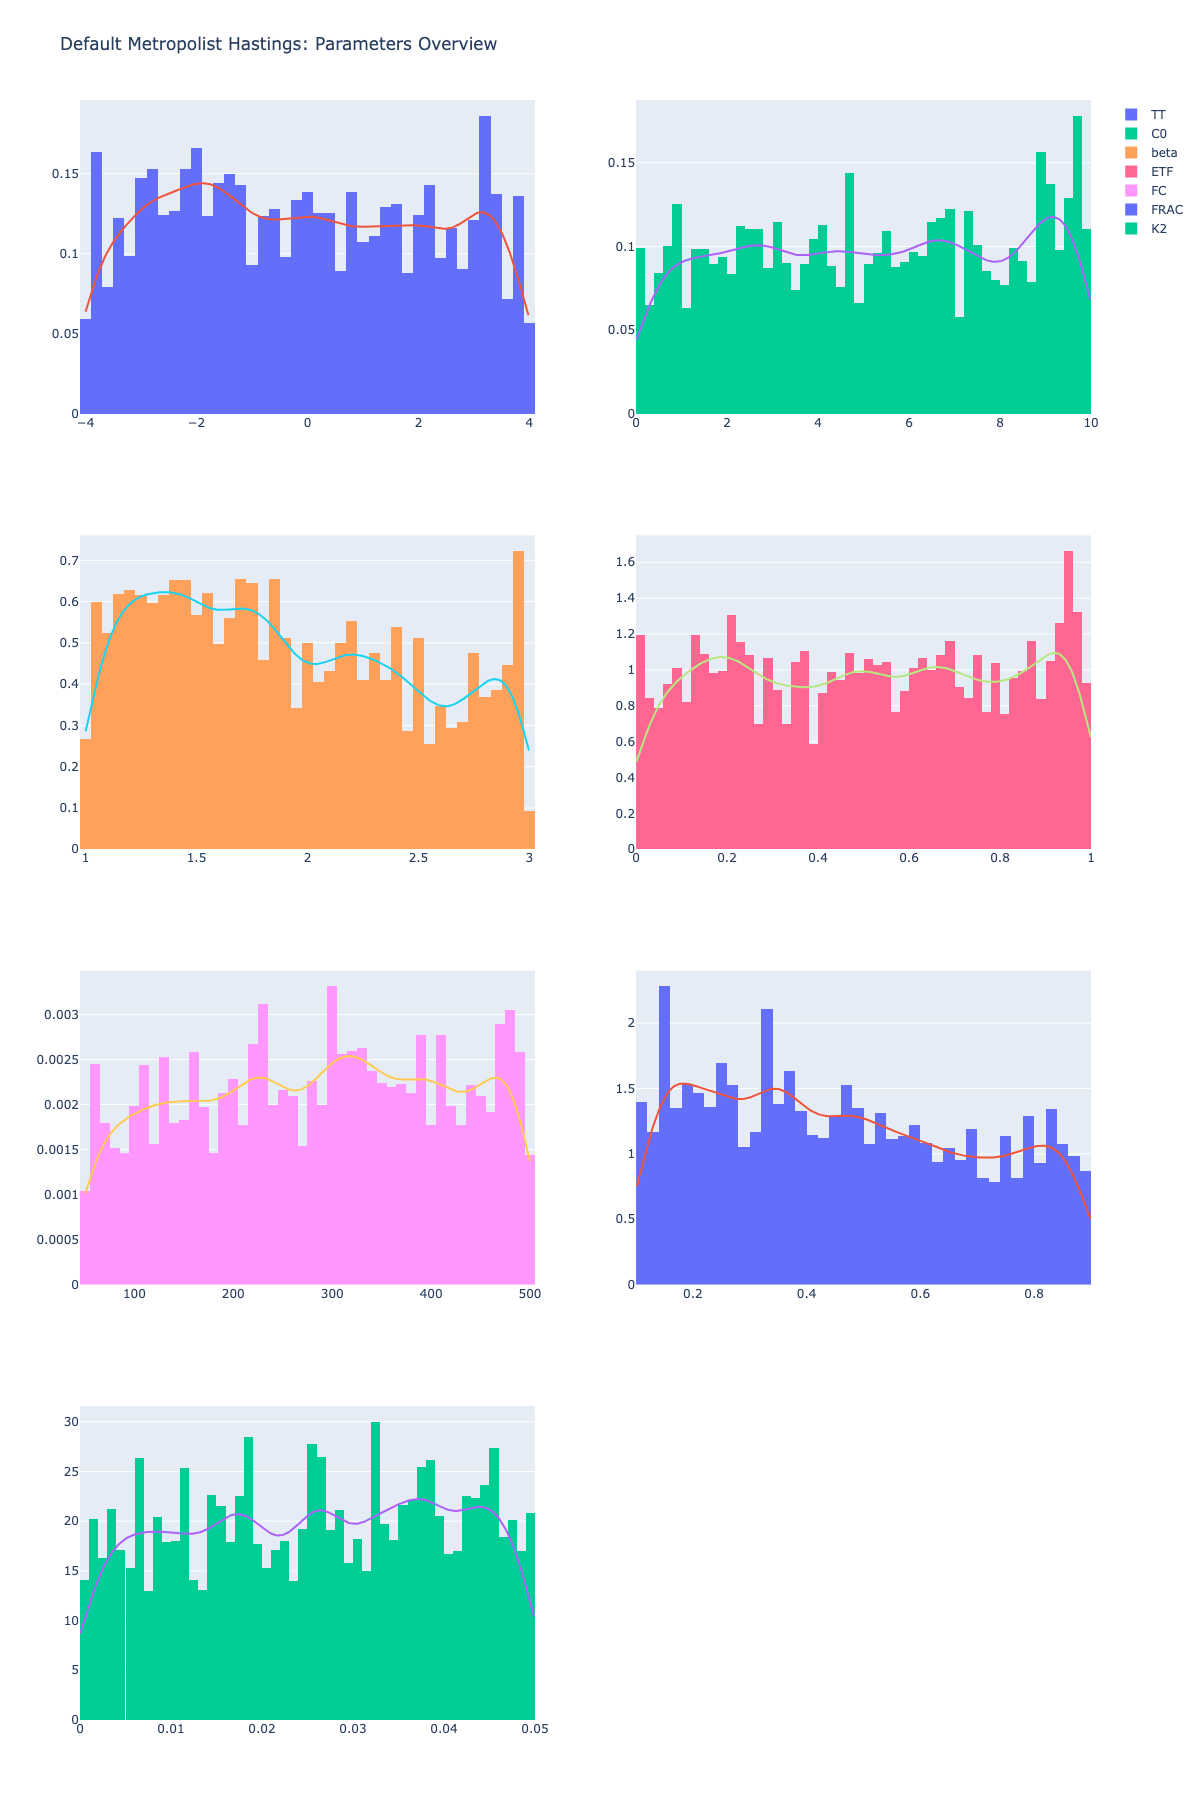
\includegraphics[width=1\textwidth]{figures/basic_mh/default_mh/default_mh_parameters_overview.png}
    \captionsetup{width=.8\textwidth}
    \caption{Overview of the posterior distribution of the parameters calibrated by the default Metropolis-Hastings algorithm}
    \label{fig:enter-label}
\end{figure}



\begin{figure}[H]
    \centering
    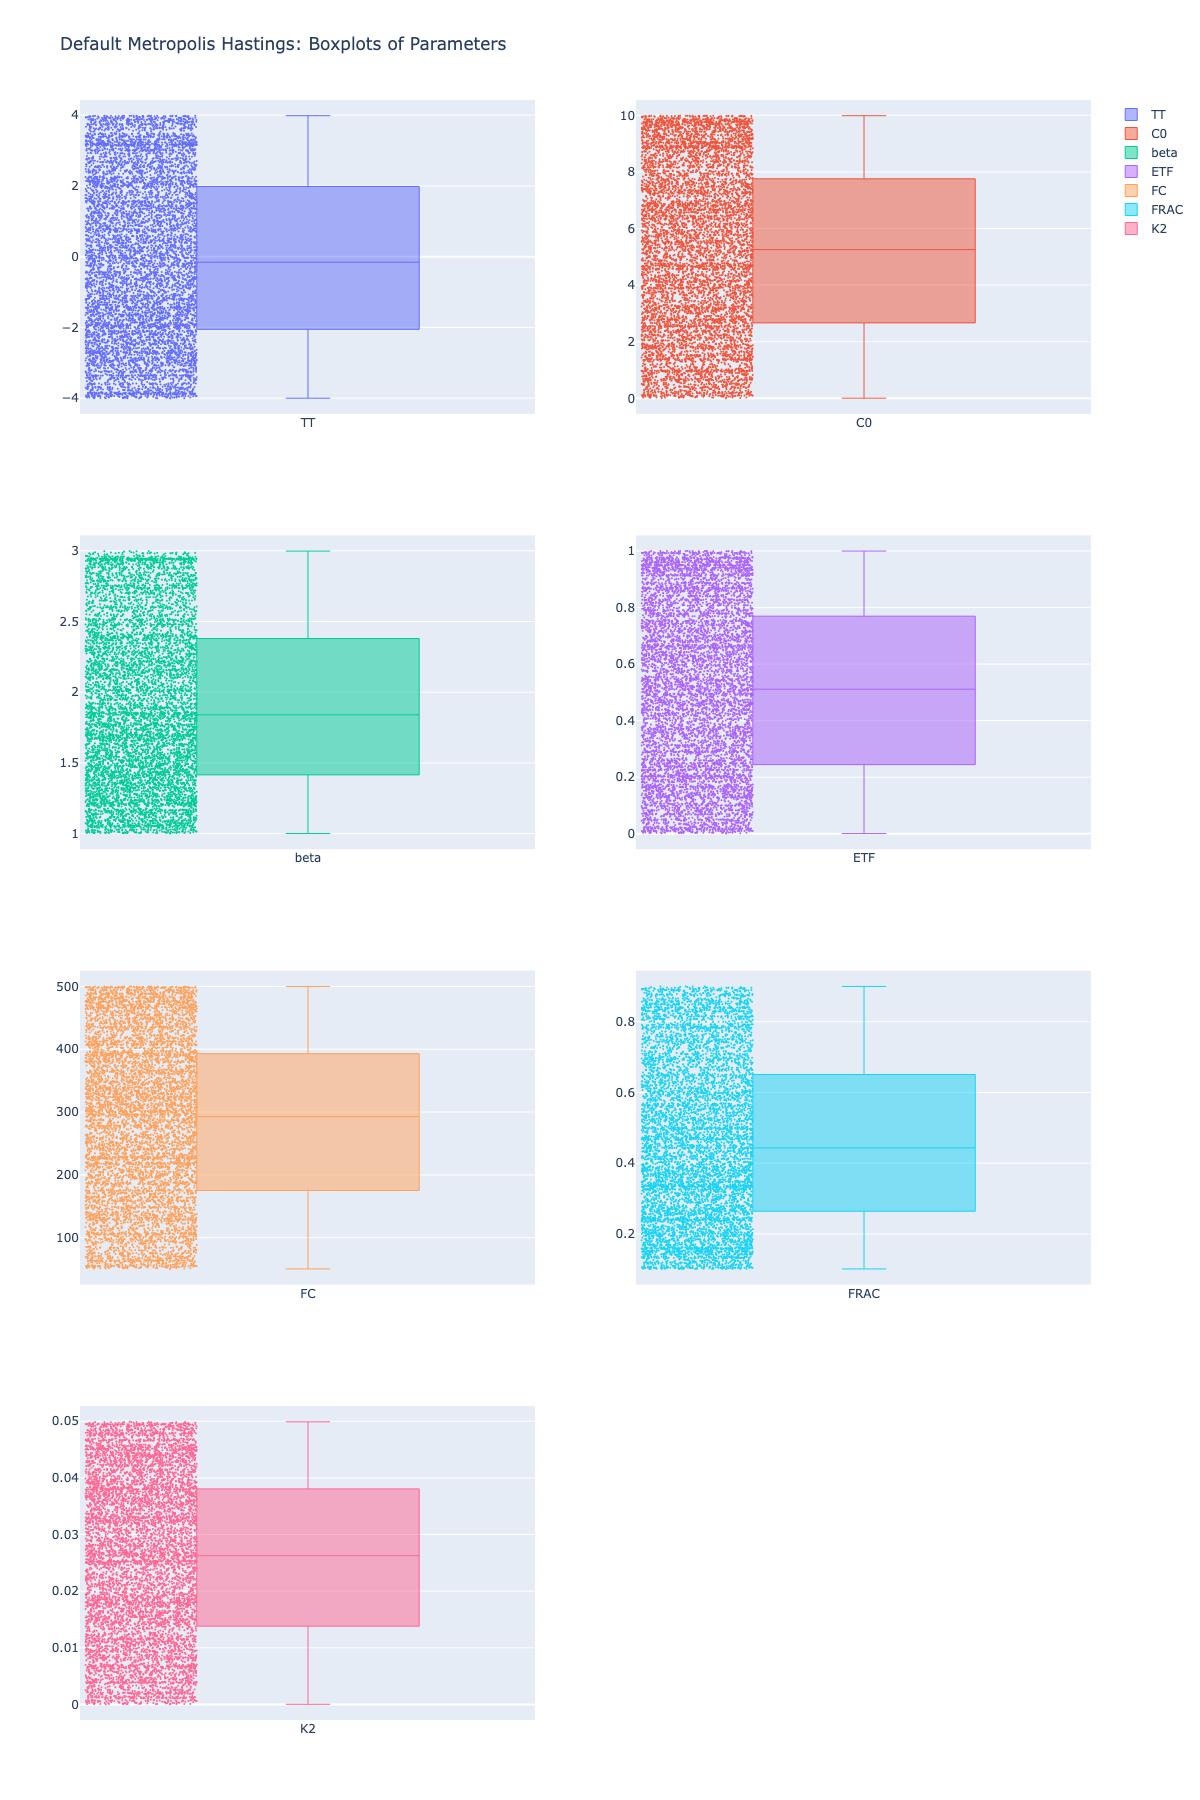
\includegraphics[width=1\textwidth]{figures/basic_mh/default_mh/default_mh_boxplot.png}
    \captionsetup{width=.8\textwidth}
    \caption{Boxplots of the generated posterior samples of each parameter calibrated by the default Metropolis-Hastings algorithm}
    \label{fig:enter-label}
\end{figure}



After analyzing the parameters individually and as a group, the result that is computed by the posterior of the Bayesian inference is revealed in Figure 5.3 and compared to the observed data. The calculated result resembles the actual measured data, particularly the posterior mean. It reaches its peak in the same period as the measured data, whereas it shows stable behavior for the rest of the time, just like the the measured data. The posterior max shows slightly more extreme behaviors at certain points. Both of the posterior time series show significant improvement based on the prior mean. 


\begin{figure}[H]
    \centering
    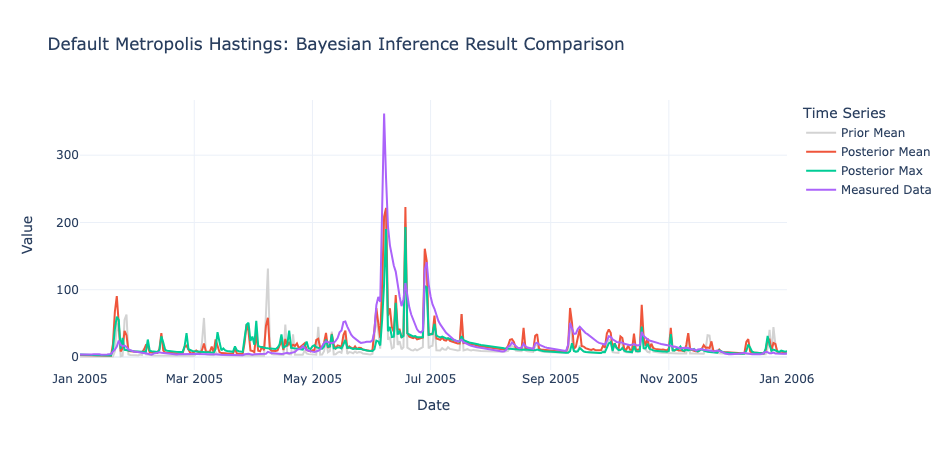
\includegraphics[width=0.7\textwidth]{figures/basic_mh/default_mh/default_mh_bayes.png}
    \captionsetup{width=.8\textwidth}
    \caption{Comparison of Bayesian inference results of the default Metropolis-Hastings}
    \label{fig:enter-label}
\end{figure}

After visualizing the parameters, we take a look at the accuracy of the data. For this part, the RMSEs and MAEs are calculated. The RMSE of the posterior mean is 22.14475485613421 and the MAE of the posterior mean is 11.399487080387862. From the graph, we can see that a significant difference in the results is shown around the peak, which might contribute to the relatively high MAE and a decent value of RMSE. The RMSE of the posterior max is 26.72454579307846 and the MAE of the posterior max is 13.196081237340492. They do not show too many differences from the posterior means, which means that the posterior distribution is relatively stable. 

These values will be later compared to the results after the input algorithm parameters exploration. In the following sections, we are going to explore specific parameters of the Metropolis-Hastings algorithm to achieve maximum accuracy. Besides, the efficiency will also be taken into account, where the run time of the algorithm will be observed and compared.


\section{Input Algorithm Parameters Exploration}
After finding the appropriate values by knowledge-based selection, all of the input algorithm parameters will be explored in this section. By trying out different reasonable values as input and interpreting the accuracy and efficiency results, we might be able to figure out a specific relation between the different input values against the accuracy or the efficiency score. Later on, the algorithm will be run using the set of input algorithm parameters which delivers the best performance by accuracy and efficiency metrics and be compared with the input algorithm parameters by knowledge-based selection on the testing data.

\subsection{Sampling Out of Bounds}
While executing this algorithm for the hydrological model, however, there is a certain issue. Since no specific information regarding the distribution is given, we are required to use the uniform distribution to describe the parameters that need to be calibrated. Since the uniform distribution ranges from a certain lower bound to a certain upper bound, it does not have an unlimited range. In this case, there is a possibility that the newly generated samples are out of bounds, which is not helpful for the calibration. For example, if a generated point, which is accepted, is out of bounds, the $p$ variable in the algorithm will be set to 0, which causes invalid values like negative infinity to occur in the calculation while using logarithm likelihood functions. If these values are sampled and carried on, values that are further from the bounds may be going to be sampled, which leads to mistakes in the result. Therefore, measures need to be taken to avoid these errors from happening. Three implementation variants against this issue have come up. These are ignoring, boundary aggregation, and reflecting boundary.

The ignoring method is the default method and the most straightforward: Any points that are generated outside of the bound are going to be eliminated. It is extremely important to mention that instead of taking another sample from the iteration, the last generated sample needs to be carried on. Since the sample out of bounds is supposed to be an impossible case, the acceptance rate in that point needs to be treated as 0, which means that this point is directly rejected. For multivariate distribution, a set of data points needs to be rejected entirely at once if one single data point is out of bounds since the acceptance rate otherwise would be different. Otherwise, the detailed balanced condition could be violated, as the transition probabilities would not be symmetric anymore for every single parameter.

The boundary aggregation method is different in treating the out-of-bounds samples, in which it transforms the sampled data that are out of bounds. We simply sample the upper bound or the lower bound and carry on from there. If a new sample is generated based on the normal distribution that is centered around the out-of-bounds sample, there is less or equal to fifty percent chance that the newly generated point is inside the range~\cite{gaussian_distribution_property}. The main benefit of this method is that there is still a minimum of fifty percent chance that the next sample is kept inside the bound in cases where the samples are out of bounds. For multivariate distribution, a single data point in each dimension can be handled individually, however, the acceptance rate needs to be calculated based on the transformed sample points. 

The posterior that is derived from the boundary aggregation method is shown in Figure 5.4.  A few samples are getting aggregated on both sides of the boundaries. If we ignore these two bars on both sides, the distributions of the rest of the samples of each parameter still resemble uniform distributions, which does not provide a lot of information regarding the actual distribution of the parameter. 

The boxplot of these samples is shown in the Figure 5.5. An obvious takeaway from this chart is that all of the boxplots have a lower first quantile and a higher third quantile, whereas the median is retained almost at the same place. The disposition of both of these quantiles is the result of the aggregation of samples on both sides of the boundaries.


\begin{figure}[H]
    \centering
    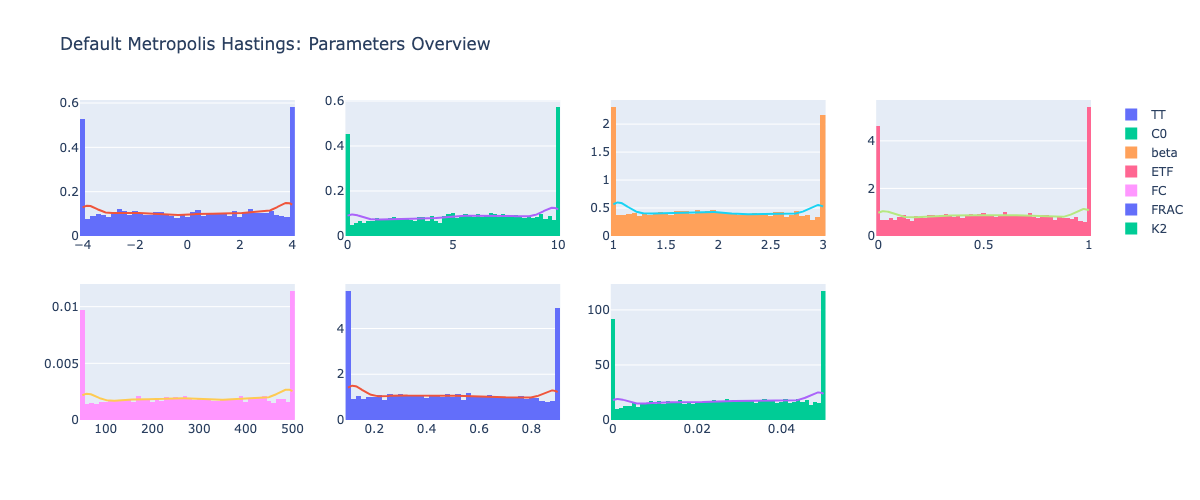
\includegraphics[width=1\textwidth]{figures/basic_mh/aggr_mh/aggr_mh_parameters_overview.png}
    \captionsetup{width=.8\textwidth}
    \caption{Overview of the posterior distribution of the parameters calibrated by the Metropolis-Hastings algorithm that samples the bound value if the sample is out of bounds}
    \label{fig:enter-label}
\end{figure}

\begin{figure}[H]
    \centering
    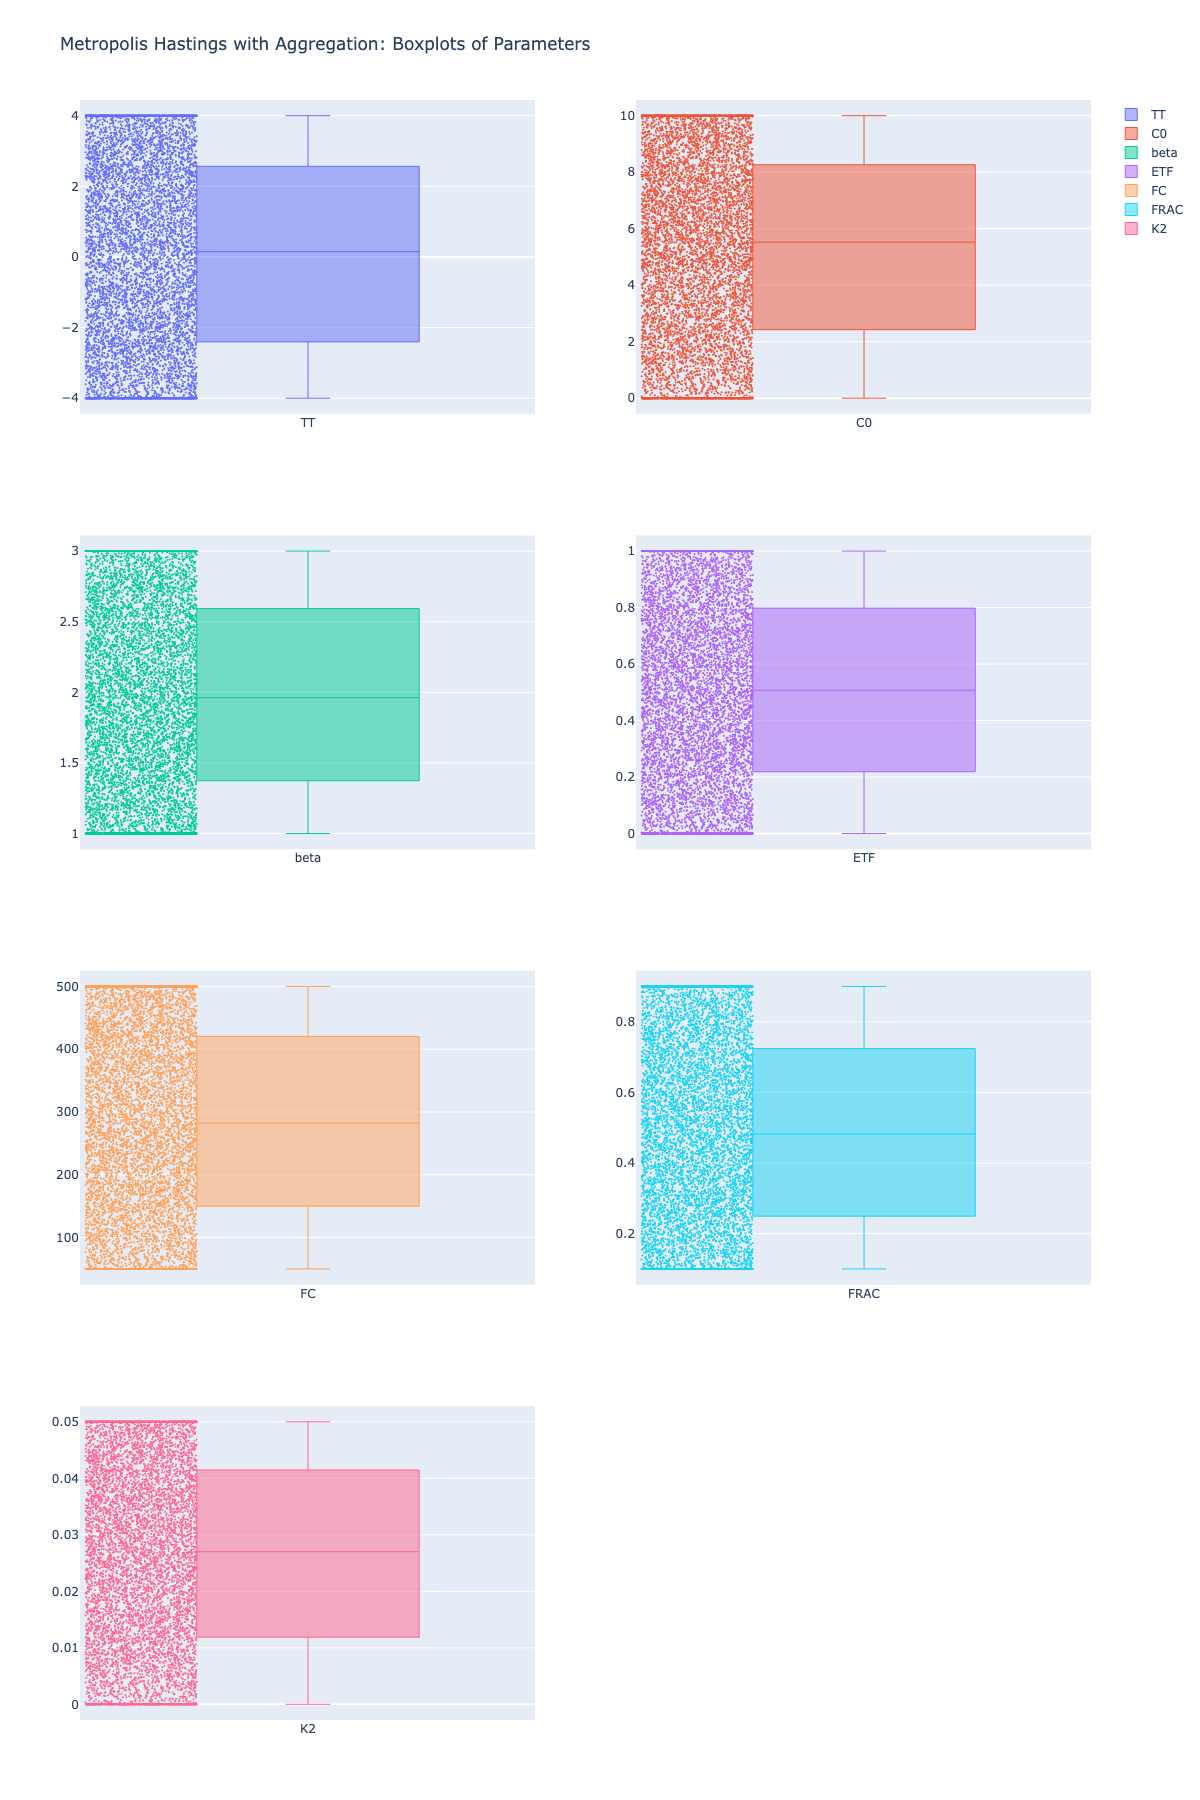
\includegraphics[width=1\textwidth]{figures/basic_mh/aggr_mh/aggr_mh_boxplot.png}
    \captionsetup{width=.8\textwidth}
    \caption{Boxplots of the generated posterior samples of each parameter
calibrated by the Metropolis-Hastings algorithm that samples the bound value if the sample is out of bounds}
    \label{fig:enter-label}
\end{figure}



The reflect boundary method also transforms the data instead of ignoring it but in a different way than the aggregation method. Due to the symmetry of the transition kernel, the possibility of sampling an out-of-bounds sample is the same as the possibility of sampling the point symmetric over the mean of the Gaussian normal transition kernel~\cite{gaussian_distribution_property}. In this case, the acceptance rate of the transformed sample point is not changed, which has no interference with the algorithm itself and future samples. For multivariate distribution, a single data point in each dimension can be handled individually and the acceptance rate does not need to be recalculated due to the symmetry of the transition kernel distribution. 

We now take a look at the posterior distribution of the samples. It is shown in Figure 5.6. From the graph, we can see that the posterior distributions sampled from this version of Metropolis-Hastings look very much different from the others. All of these posterior distributions resemble normal distributions, with one peak somewhere in the middle. For some parameters like C0, beta, ETF, and TT, the boundary is shifted, which means that no samples from the region near the boundaries are generated. Since all of the samples that are out of bounds are reflected, the reflected samples compensate the holes of the non-reflected samples, so that it gives rise to a normal distribution like posterior.

\begin{figure}[H]
    \centering
    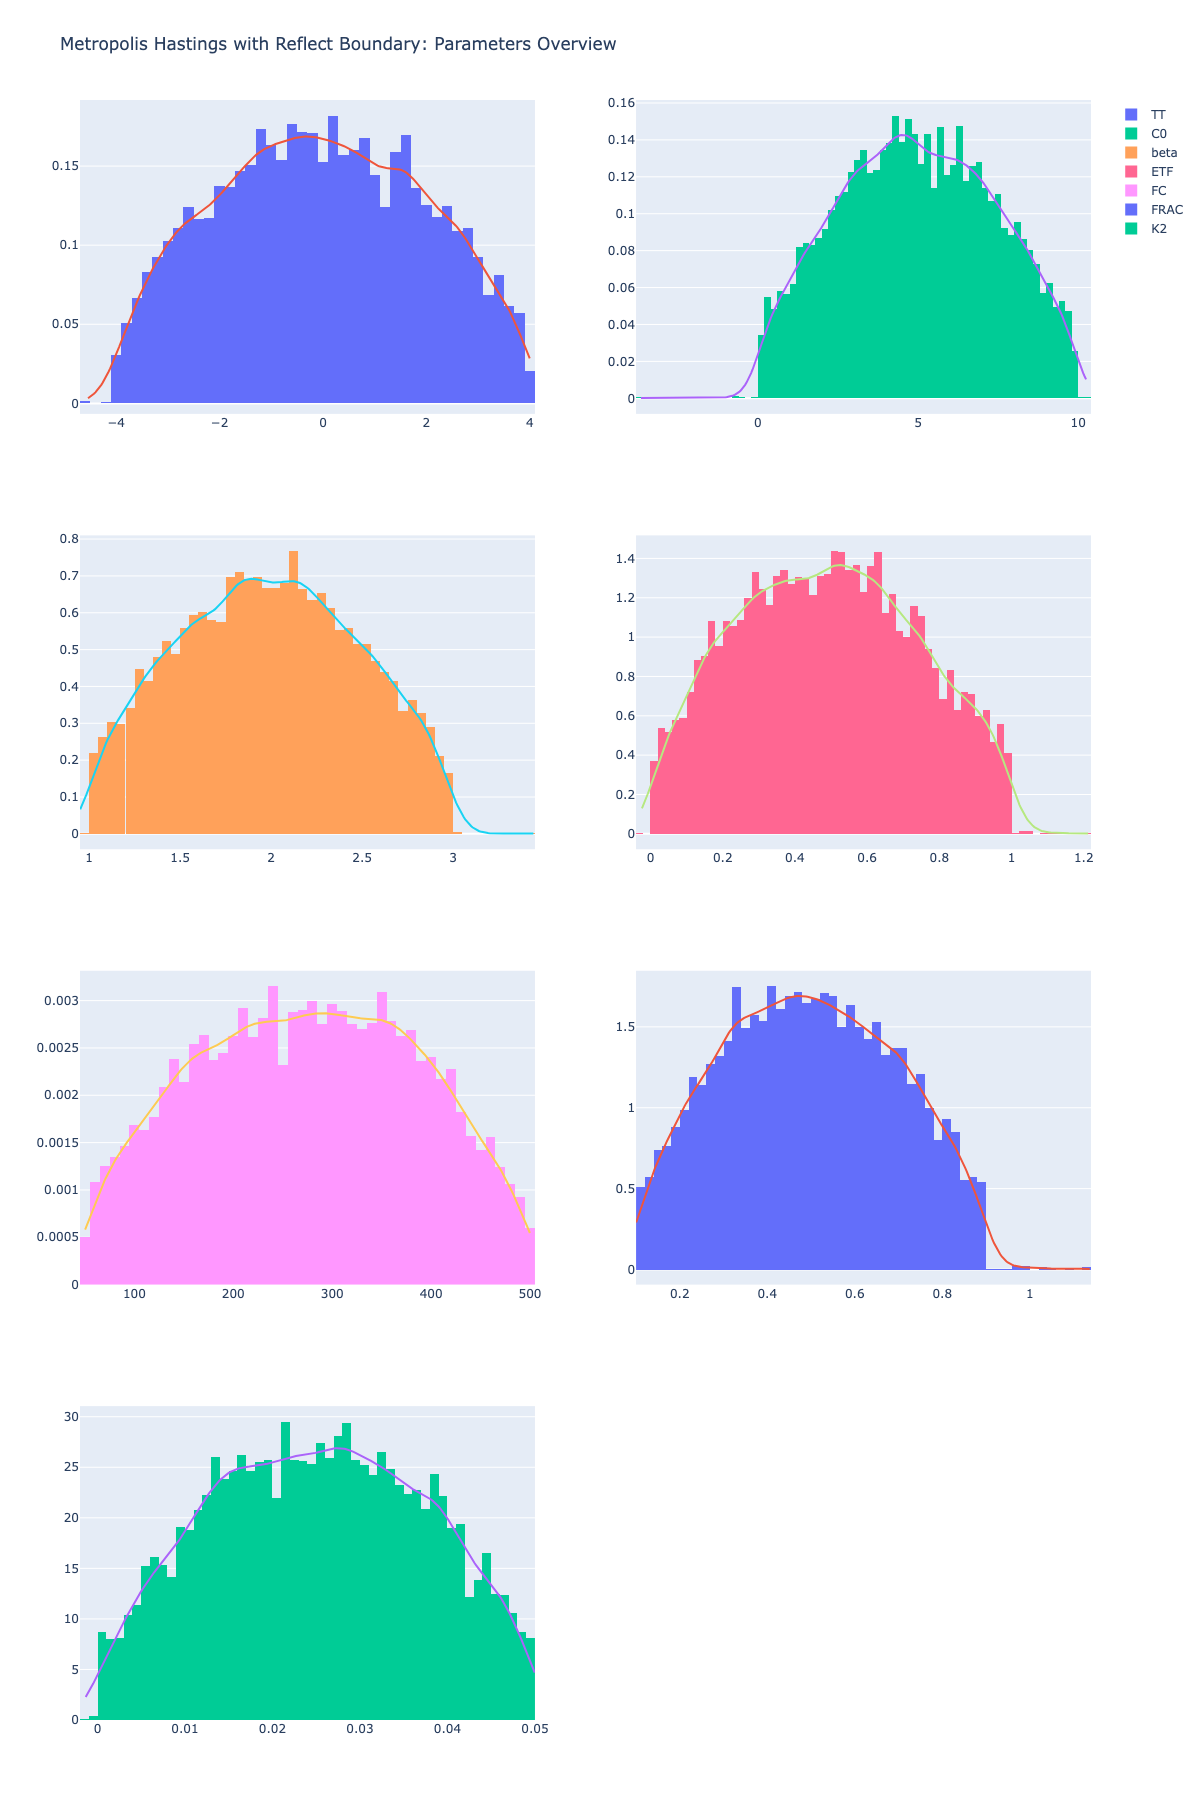
\includegraphics[width=1\textwidth]{figures/basic_mh/rb_mh/rb_mh_parameters_overview.png}
    \captionsetup{width=.8\textwidth}
    \caption{Overview of the posterior distribution of the parameters calibrated by the Metropolis-Hastings algorithm that reflect the samples into the inside of the range if the they are out of bounds}
    \label{fig:enter-label}
\end{figure}

The boxplots of the parameters are shown in Figure 5.7. Due to the normal distribution like posterior, all of the boxplots shrink by a certain amount, with some having lower upper bounds or upper lower bounds. This is an apparent result, since the shape of the normal distribution focuses on the mean, whereas the sampling probabilities of samples that are further from the mean are lower. This property can be presented by the boxplots.

\begin{figure}[H]
    \centering
    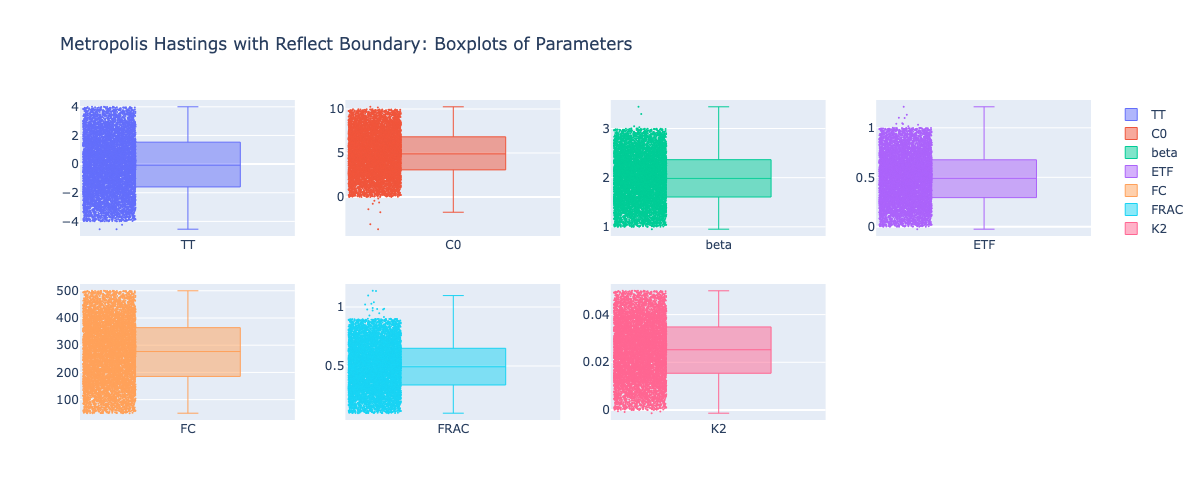
\includegraphics[width=1\textwidth]{figures/basic_mh/rb_mh/rb_mh_boxplot.png}
    \captionsetup{width=.8\textwidth}
    \caption{Boxplots of the parameters calibrated by the Metropolis-Hastings algorithm that reflect the samples into the inside of the range if the they are out of bounds}
    \label{fig:enter-label}
\end{figure}



To find out which of these three variants delivers the best result, each of these three versions is separately executed, while all of the rest input algorithm parameters are set to the same value or instance. The different metrics that are mentioned in the section above are then calculated and visualized using a bar chart so that the values can be compared. The result is shown in Figure 5.8. The first impression of the bar chart is that the accuracy of the actual inferred results is pretty similar among all three versions, with the ignoring and the aggregate methods performing only slightly better. For efficiency, however, the ignoring performs better than both of the other methods by a huge margin. The reason behind it is obvious: the ignoring operation is way more efficient than the reflecting boundary and aggregation, which involves mathematical operations. Therefore, the default ignoring method is the clear winner here and should be retained for further model executions.


\begin{figure}[H]
    \centering
    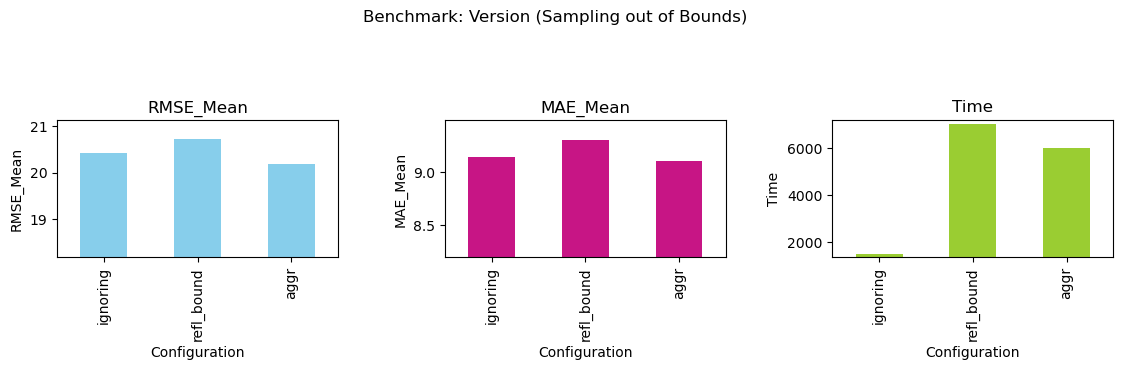
\includegraphics[width=1\textwidth]{figures/basic_mh/benchmark/sampling_otb.png}
    \captionsetup{width=.8\textwidth}
    \caption{Comparison of the accuracy and the efficiency of Metropolis-Hastings algorithms based on the technique of handling samples generated out of bounds}
    \label{fig:enter-label}
\end{figure}



\subsection{Sampling Kernel}
The sampling kernel plays a crucial role in the accuracy and efficiency of the performance. Since we stick to the normal distribution in this paper, the standard deviation is the only value that needs to be explored. As suggested in the above section of 5.2, the default value of the standard deviation is set to $6$ because it is the largest possible number that fits in the use case of the hydrology model. However, the final result would also be different if the standard deviation is less than the optimal one. In this case, the movement of the samples is going to be relatively centered local, since the points in the vicinity of the mean are more likely to be sampled. To test multiple scenarios and their behaviors, three values for the standard deviation are going to be tested in the following execution: the range interval over $8$, over $10$, over $12$, over $18$, and over $24$.

\begin{figure}[H]
    \centering
    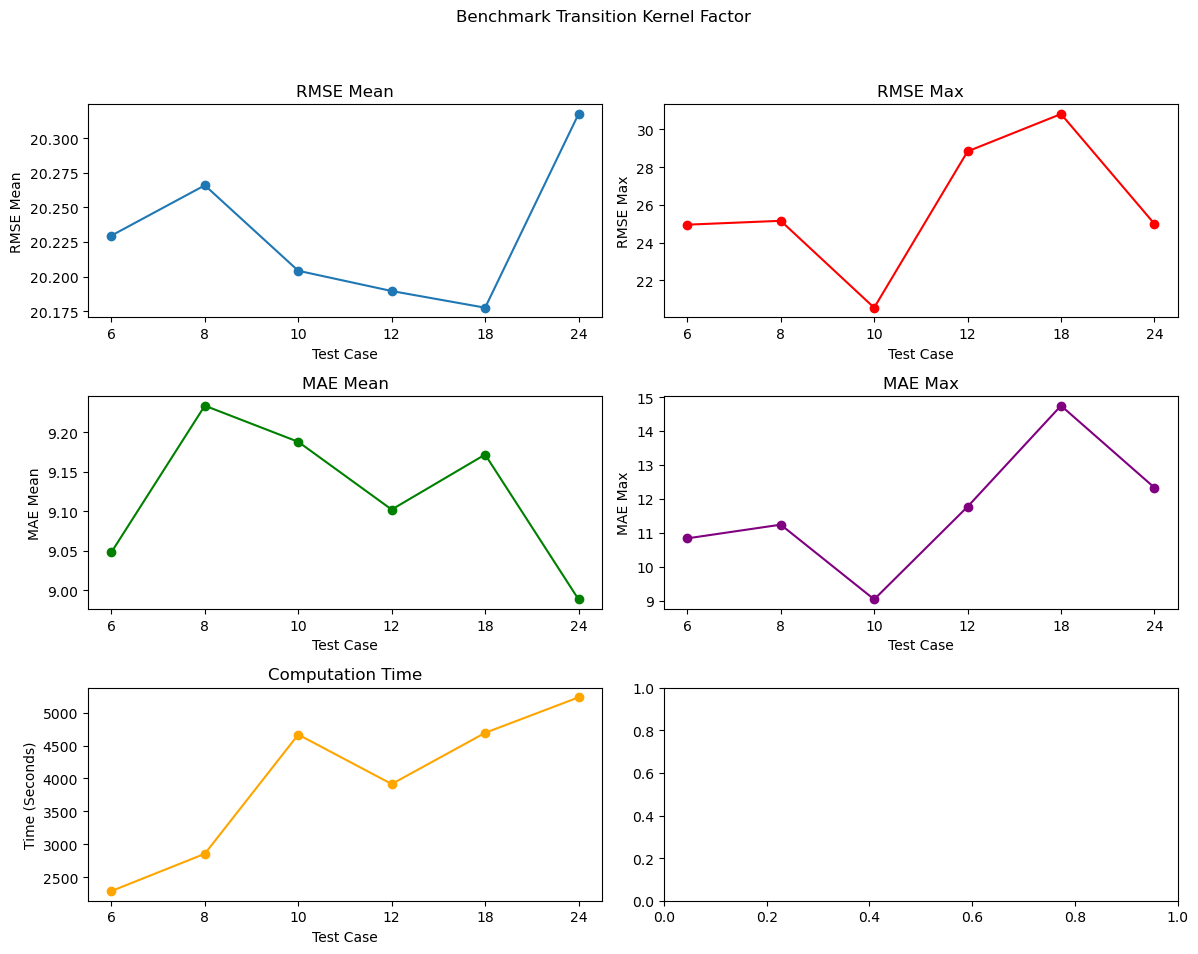
\includegraphics[width=1\textwidth]{figures/basic_mh/benchmark/sensitivity_transition.png}
    \captionsetup{width=.8\textwidth}
    \caption{Comparison of the accuracy and the efficiency of Metropolis-Hastings algorithms based on the sampling kernel standard deviation}
    \label{fig:enter-label}
\end{figure}

The result shows a certain level of dependency between the accuracy metric and the input values. For both accuracy metrics, the accuracy scores the input value do not differ that much from each other, which indicates that the sampling kernel factor is irrelevant for the accuracy result. For the computation time, on the other hand, there is an exponential relationship between the run time and the sampling kernel value, with an exception of the test case $10$ as anomaly. In conclusion, a lower value such as $6$ for the sampling kernel factor would be optimal due to the efficiency of the algorithm.

\subsection{Likelihood Functions}
At the start of the chapter, we have already discussed the importance of the role played by standard deviations in the likelihood functions. As mentioned before, $1$ is selected for the default value. However, the choice of the standard deviation does impact the final result, since it exerts an influence on the sampling probability of the values based on their distance from the mean. If the standard deviation is set lower, the sample that is away from the mean will receive less probability. If the standard deviation is set higher, that sample will not receive that little probability, which allows more tolerance to be present in the calculation. However, the value cannot be too large, otherwise, the tolerance level will be too high for the likelihood function to give out a meaningful solution. Thus, for the test values, we go from $1$ down to $8$, which is an interval of values that still might generate meaningful calculations. The selected values for testing are $1$, $3$, $5$ and $8$. 

As we can derive from Figure 5.10, the metrics for the mean also do not differ that much from each other. In this case, the conclusion could be drawn that the standard deviation does not have a huge impact on the actual inferred result. For the inferred maximum time series, the discrepancy is also not obvious, even though the test case $5$ shows the most instability throughout the posterior. Nevertheless, using the test case $5$ results in the most efficient calculation, whereas using the test cases $1$ and $2$ will require slightly more computation time.


\begin{figure}[H]
    \centering
    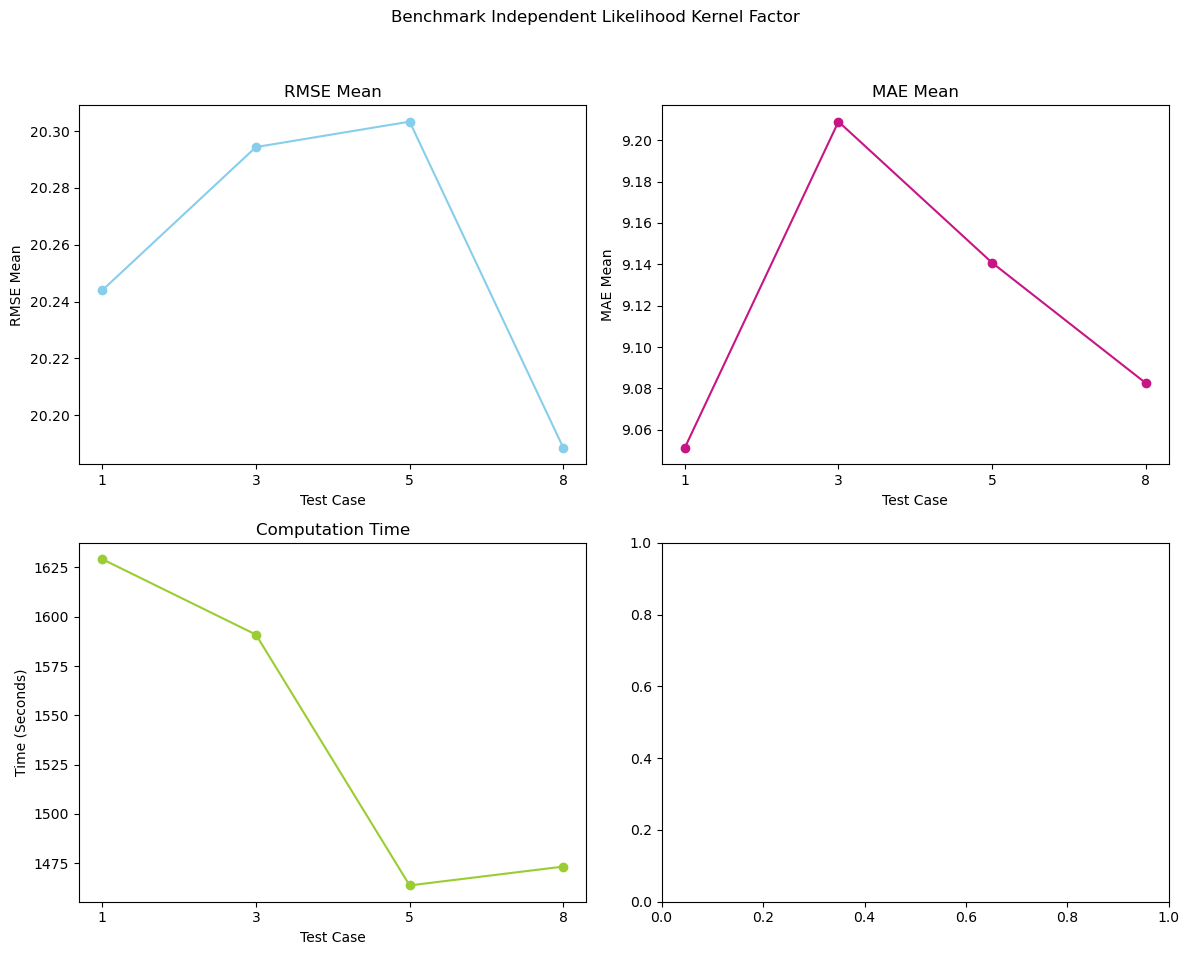
\includegraphics[width=1\textwidth]{figures/basic_mh/benchmark/sensitivity_likelihood_independent.png}
    \captionsetup{width=.8\textwidth}
    \caption{Comparison of the accuracy and the efficiency of Metropolis-Hastings algorithms based on the likelihood function standard deviation}
    \label{fig:enter-label}
\end{figure}



The above-computed likelihood function takes in a value as the standard deviation so that each sample is independently observed from another. Another alternative implementation to the dependent likelihood function would be the dependent likelihood function, which takes in the observed data as the standard deviation. This technique is common in the hydrological field~\cite{dream}, which uses the observed data as the standard deviation for a better understanding of the relationship between the inferred and observed data, therefore a precise likelihood calculation. Since the observed data might be too large for the likelihood function to deliver meaningful results, an alternative way is to take a certain factor of the observed data as input. Here, several factors are going to be tested, including $0.2$, $0.4$, $0.6$ and $0.8$. The goal is to observe the correlation between the accuracy and the value as it increases.


The result is shown in Figure 5.11, where we see a pattern: the accuracy of the inferred data decreases as the factor increases. As for the computation time, the case of $0.6$ requires the most time to perform computation, and is, however, still pretty similar to the rest. Therefore, the case $0.2$ should be the optimal choice.

\begin{figure}[H]
    \centering
    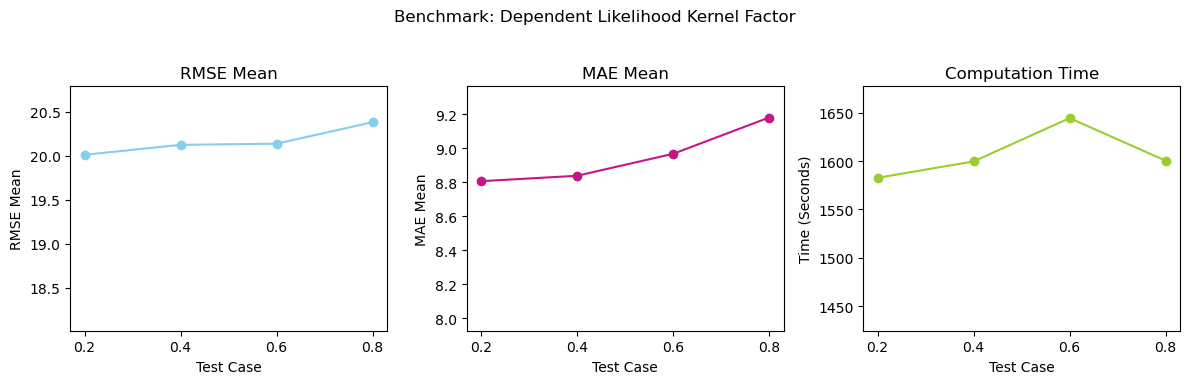
\includegraphics[width=1\textwidth]{figures/basic_mh/benchmark/sensitivity_likelihood_dependent.png}
    \captionsetup{width=.8\textwidth}
    \caption{Comparison of the accuracy and the efficiency of Metropolis-Hastings algorithms based on the dependent likelihood function standard deviation}
    \label{fig:enter-label}
\end{figure}


Comparing the dependent and the independent version of the likelihood functions, the dependent version with a standard deviation of $0.2$ times the measured data outperforms the independent version with a standard deviation of $5$, despite a slightly longer run time, which is reasonable due to the mathematical computation of the standard deviation. The incorporation of exact data in the likelihood function does provide a more accurate result.

\subsection{Alternative Implementation of Probability Acceptance Rate}
After we explore both of the input algorithm parameters that are responsible for the calculation of the acceptance rate, we move on to the selection of the acceptance rate. As mentioned above, two choices are available for the acceptance rate calculation: One option is that we take the mean of all the values as an acceptance rate, so that the final acceptance rate could more generally represent all of the individual acceptance rates by parameter. Another option is to take the maximum value of the entire acceptance rate array. On the one hand, we can improve the efficiency of the algorithm, since the calculation of the mean is avoided. On the other hand, some dimensions might be easier to sample from than others due to less complexity. Using the maximum acceptance rate gives us therefore the insight of the entire parameter space, where the parameter with the best performance decides the acceptance rate. However, the maximum acceptance rate might be misleading if the distribution of the acceptance rate array is too widespread, which results in the complete opposite of efficiency and accuracy.

We execute the algorithm in both versions, with the rest of the parameters being identical. Figure 5.12 suggests that for the HBV-SASK model, the mean sampling method does not only deliver a slightly better performance in accuracy but also more stability and most importantly: better efficiency. This shows that the acceptance rate in each iteration in the array might have far different values so the max sampling method cannot deliver good enough results. Therefore, we stick to the original mean sampling method.


\begin{figure}[H]
    \centering
    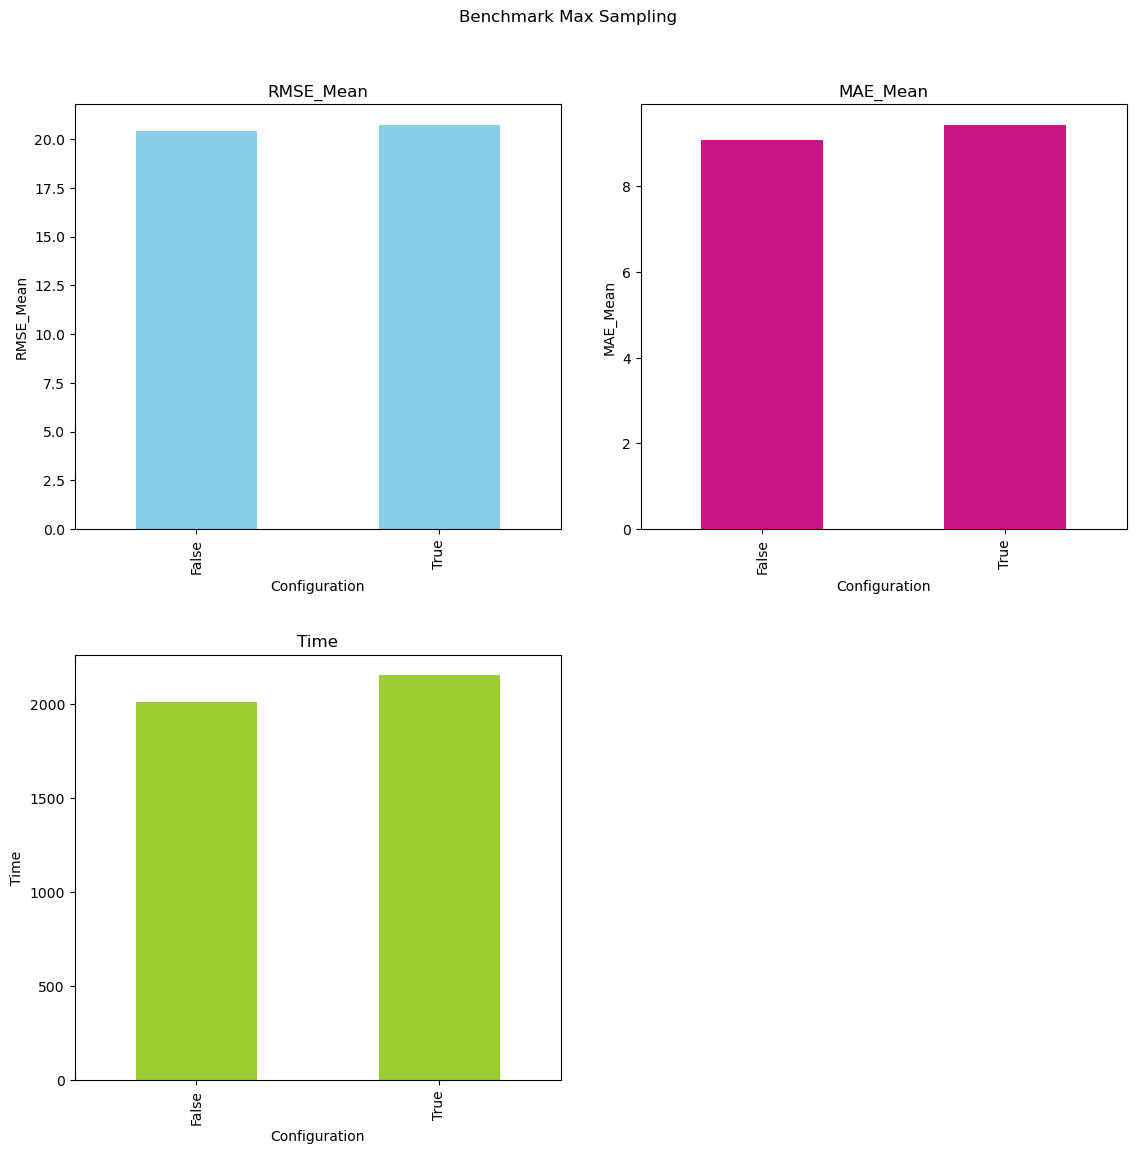
\includegraphics[width=1\textwidth]{figures/basic_mh/benchmark/max_sampling.png}
    \captionsetup{width=.8\textwidth}
    \caption{Comparison of the accuracy and the efficiency of Metropolis-Hastings algorithms based on the implementation of probability acceptance rate calculation}
    \label{fig:enter-label}
\end{figure}



\subsection{Burn In Phase}
Another crucial part of all Markov chain Monte Carlo algorithms is the discard of the burn-in phase. For Metropolis-Hastings, it is no exception. Determining a general optimal burn in phase leads to an optimization of the result since it is the process of removing generated samples that do not follow the stationary distribution and are unstable. The algorithm was previously executed with a burn-in phase of 20 percent, which means that the first twenty percent of the generated sample data are discarded. However, a comparison to other values of the burn-in phase would give us an overview of how effective the 20 percent is and whether it is enough. The values that are used for comparison are $33$ and $50$ percent. On the graph, the values $2$, $3$, and $5$ denote the denominator of the burn in phase, as they should be interpreted as $\frac 1 2$, $\frac 1 3$ and $\frac 1 5$.

Figure 5.13 infers that the case $50$ percent and the case $20$ percent show relatively similar accuracy and efficiency. However, because removing half of the samples might be a bit too much and the similarity in performance, $20$ percent is a better choice. Therefore, for the rest of the execution phase, we keep discarding the first $20$ percent of the samples as the burn-in phase.

\begin{figure}[H]
    \centering
    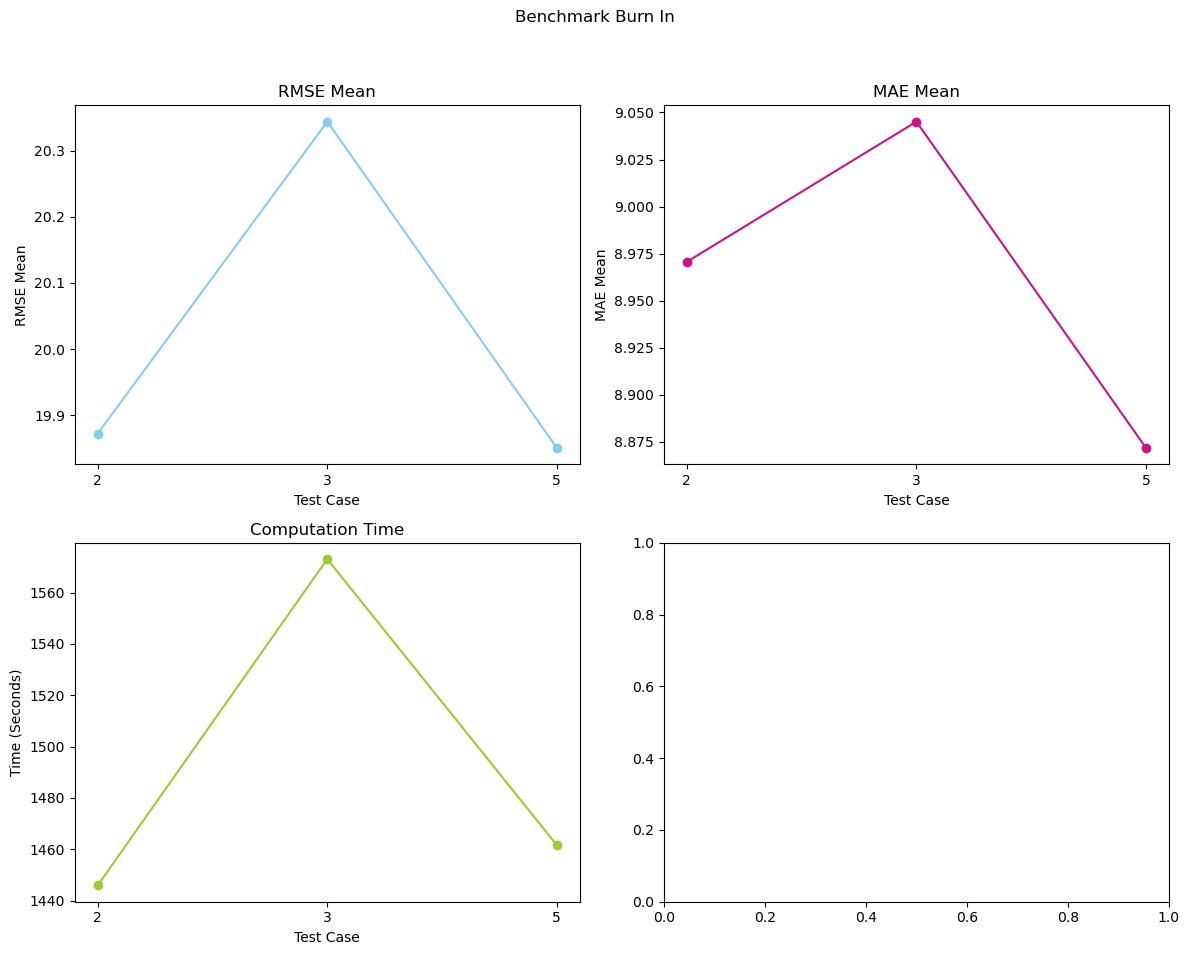
\includegraphics[width=1\textwidth]{figures/basic_mh/benchmark/burnin_factor.png}
    \captionsetup{width=.8\textwidth}
    \caption{Comparison of the accuracy and the efficiency of Metropolis-Hastings algorithms based on length of burn in phase}
    \label{fig:enter-label}
\end{figure}

\subsection{Effective Sampling Size}
Effective sampling size is a new concept that has not been introduced in this paper until here. It generally indicates the number of samples that are independent from each other. A basic way to implement an effective sampling size in the Markov chain Monte Carlo algorithms is to skip a few samples and only regard every several samples in our sample space. The reason to do this is that in Markov chain Monte Carlo algorithms, every sample is dependent on the last sample generated. However, this dependency might have a higher degree of influence, for instance: the newly generated sample is most likely to lie inside of a certain range depending on the standard deviation. Therefore, not considering the sample directly after another might lead to a certain level of independence, which gives rise to more generalization of the sampling space. 

For testing purposes, we compare the algorithm that does not include the effective sampling size feature with algorithms that only consider every second, third, fourth, and fifth sample for the sampling space. The result is shown in Figure 5.14. The efficiency is proportional to the value set for the effective sample size, whereas no pattern could be found for the accuracy aspect. Even though only considering the third sample is relatively less efficient than considering every second sample or even not implementing this feature, it provides better accuracy than all the other cases and relatively better stability due to the low RMSE and MAE of the maximum time series. Therefore, it would be wise for us to keep retaining only the third value from the sample space in the later execution of the Metropolis-Hastings algorithm.

\begin{figure}[H]
    \centering
    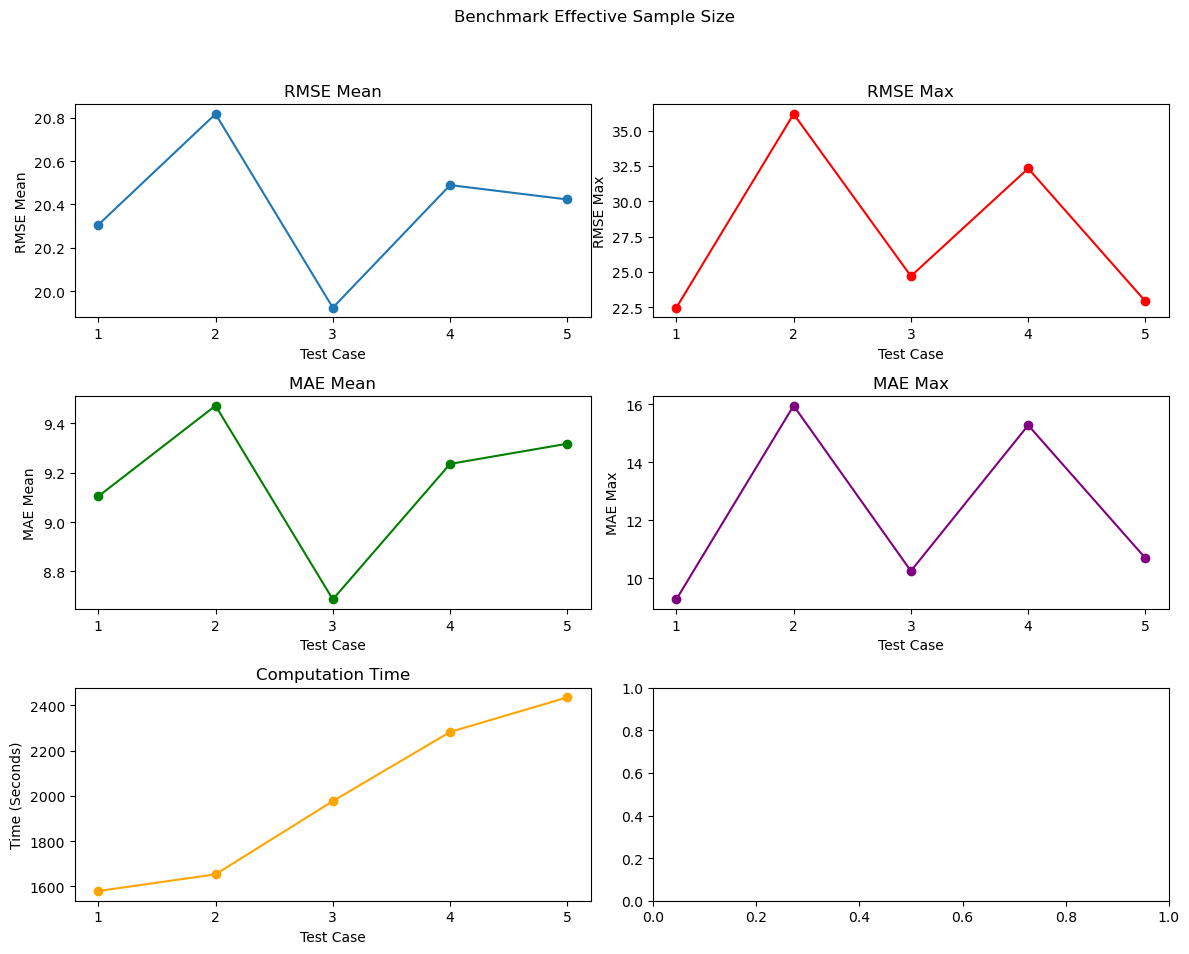
\includegraphics[width=1\textwidth]{figures/basic_mh/benchmark/effective_sample_size.png}
    \captionsetup{width=.8\textwidth}
    \caption{Comparison of the accuracy and the efficiency of Metropolis-Hastings algorithms based on the selection of effective sample size}
    \label{fig:enter-label}
\end{figure}


\subsection{Iteration}
Another crucial part of the Metropolis-Hastings algorithm is the amount of iterations. More iterations mean that more samples are gathered. To understand whether the amount of samples that are gathered is enough or not, comparing the accuracy with other numbers of iterations is needed. Until now, we performed the Metropolis-Hastings algorithm with $10000$ iterations. Now we compare this number to other iterations like $5000$, $20000$, $40000$, and $80000$ to find out which number of iterations would deliver the best result and give a decent efficiency.

The result is shown in Figure 5.15, where it is clear to observe that the computation time grows proportionally to the number of iterations. The case of $5000$ delivers the best accuracy and efficiency but might lead to too small of a sample space due to the removal of the burn in period and effective sample size. Of all of the rest cases, they share a similar range of accuracy. However, due to the efficiency of run time, more than $10000$ iterations will be an overkill. Therefore, we continue to execute the algorithm with $10000$ iterations. 

\begin{figure}[H]
    \centering
    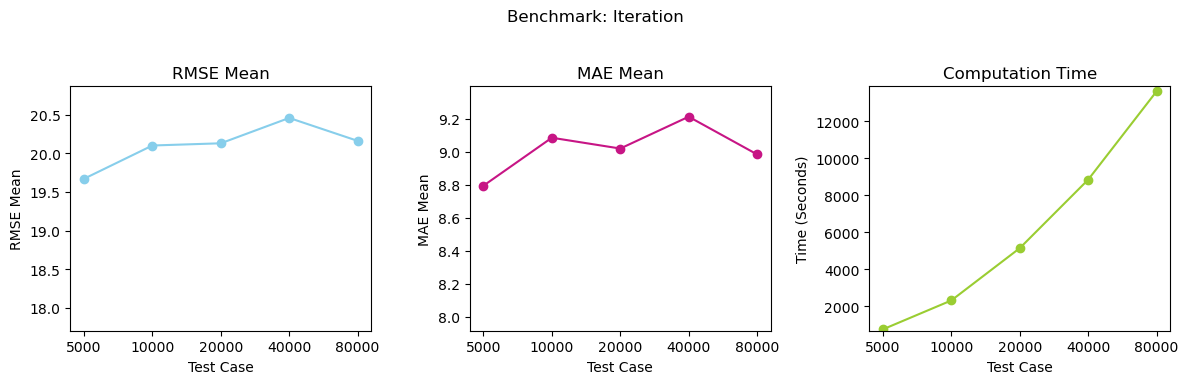
\includegraphics[width=1\textwidth]{figures/basic_mh/benchmark/iteration.png}
    \captionsetup{width=.8\textwidth}
    \caption{Comparison of the accuracy and the efficiency of Metropolis-Hastings algorithms based on the number of iterations}
    \label{fig:enter-label}
\end{figure}


\subsection{Initial States}
The last input algorithm parameter that needs to be explored is the initial states. The initial states should not have that much of an effect on the accuracy, but rather a great influence on the efficiency~\cite{mcmc_practice}. A better initial state would allow the algorithm to get rid of the burn-in phase and sample from the stationary distribution sooner, which reduces calculation burdens. It also allows the sampling kernel to discover more samples from the optimal ranges.

Several possible initial states should be taken into consideration. The most general one is the random initial state, which is used when there is little information regarding the distribution available. To do this, we sample a random state from the posterior and start from here. For testing purposes, however, we randomize 1000 samples and take the mean of them to maximize generalization and randomization. The lower and the upper boundary as the initial values would also work, which requires no initialization at all. Other possible values are derived from prior and posterior distributions. We try the first quantile, the mean, and the third quantile of the prior so that we can figure out whether an optimal starting value is coincidentally near these points. However, the focus point should be on the following three initial states: the first and the third quantile of the posterior distribution as well as the median of the posterior distribution. In the third section of this chapter, we generate a primary result that provides a general result of the posterior distribution. To start the entire algorithm from an inferred posterior state might result in better entry into the algorithm since the starting states are already proven to be very possible on the stationary distribution. Instead of taking the mean of the posterior, we select the median because it represents the half position of the entire posterior distribution, whereas the mean only represents the middle value. It is expected that the most desirable solution comes from one of the proposals of the posterior.

We execute the model with all these different initial states and receive the results shown in Figure 5.16. The RMSE and MAE of the mean time series over all of the test cases prove that the performance is not influenced by the initial states. However, the efficiencies of the algorithms with different initial states do have a massive difference between them. The maximum initialization performs well, as well as the third quantile of the prior, the third quantile of the posterior, and the median of the posterior. After checking the numerical statistics, the median of the posterior delivers the most efficiency as expected. Therefore, it will be set as the default initial state.

\begin{figure}[H]
    \centering
    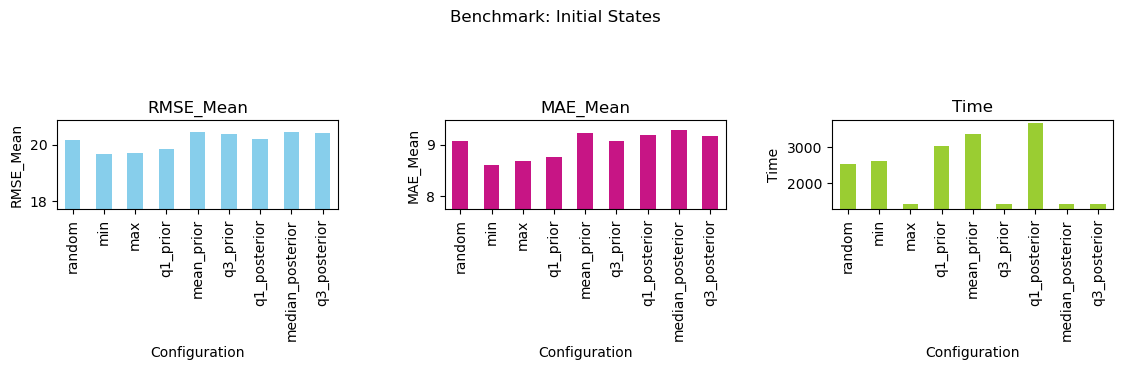
\includegraphics[width=1\textwidth]{figures/basic_mh/benchmark/init_method.png}
    \captionsetup{width=.8\textwidth}
    \caption{Comparison of the accuracy and the efficiency of Metropolis-Hastings algorithms based on the selection of initial states}
    \label{fig:enter-label}
\end{figure}


\section{Result Comparison}
After evaluating all of the input algorithm parameters, we will compare both sets of input algorithm parameters by using the Monte Carlo simulation. Using the set of input algorithm parameters that deliver the best performance by accuracy metrics in the exploration phase, which will, later on, be called the tuned input algorithm parameters, the model will be executed 1000 times, where the RMSE and the MAE of the result time series mean and maximum will be calculated. These results are going to be then compared to those of the models that run on the knowledge-based set of input algorithm parameters so that the set of input algorithm parameters that delivers better results will be selected to represent the basic Metropolis-Hastings method.

We first draw the histogram and the KDE plot for all of the parameters. It is shown in Figure 5.17. We can observe that the distributions fluctuate more than the parameters from the model that uses the knowledge-based input algorithm parameters. In this case, some of the parameters still show irregularity, whereas some of the distributions do show some certain level of resemblance to normal distribution, such as C0, FC, FRAC, and K2. Similar to the case before, the probability of sampling values near both boundaries is relatively low. 

\begin{figure}[H]
    \centering
    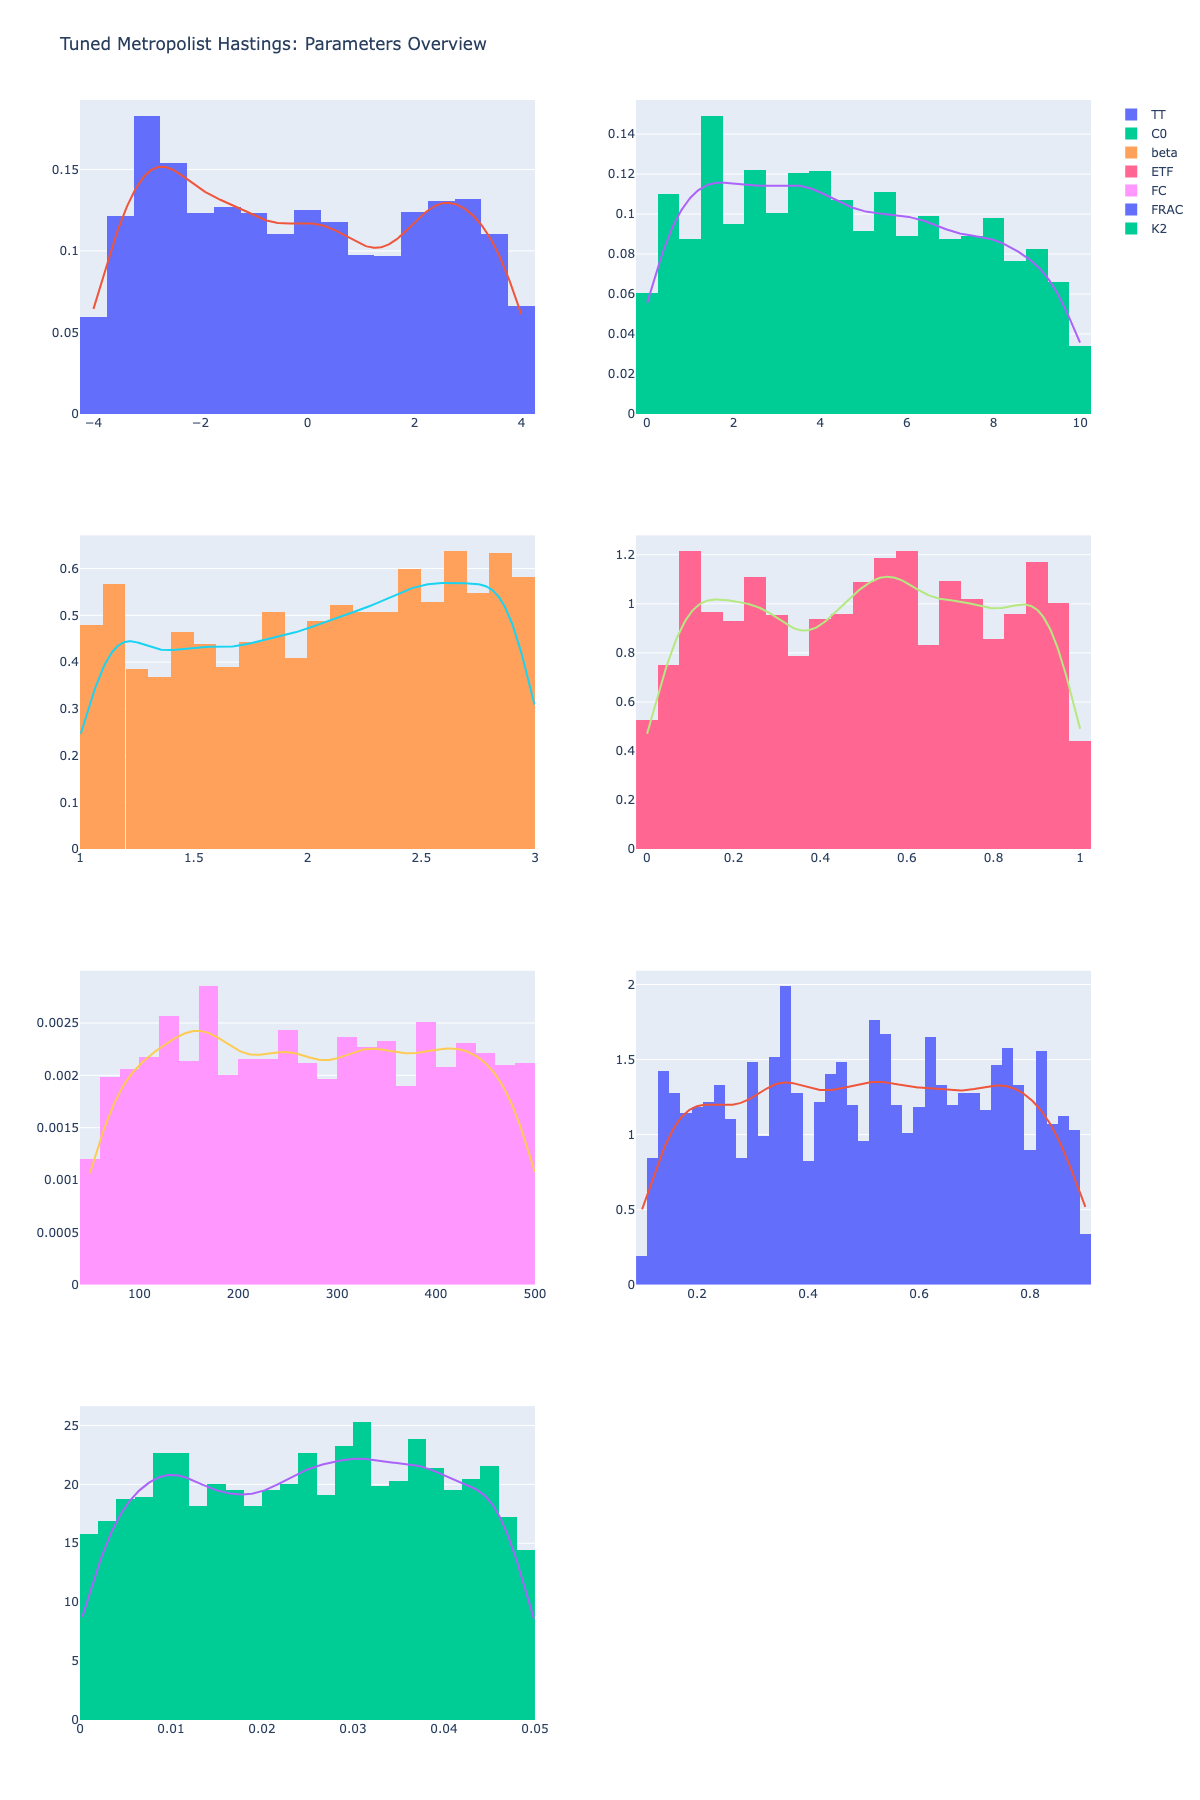
\includegraphics[width=1\textwidth]{figures/basic_mh/tuned_mh/tuned_mh_parameters_overview.png}
    \captionsetup{width=.8\textwidth}
    \caption{Overview of the posterior distribution of the parameters calibrated by the Metropolis-Hastings algorithm with tuned input algorithm parameters}
    \label{fig:enter-label}
\end{figure}


The boxplots of these parameters are shown in Figure 5.18. We can see that the ranges of most of the sampled parameters are different from the knowledge-based version. The beta and the C0 parameters have moved completely towards the lower bound, whereas the FRAC parameter has moved upwards. The ETF parameter retained its lower bound but had a lower upper bound. In contrast, The TT parameter retained its upper bound, however had a lower bound.


\begin{figure}[H]
    \centering
    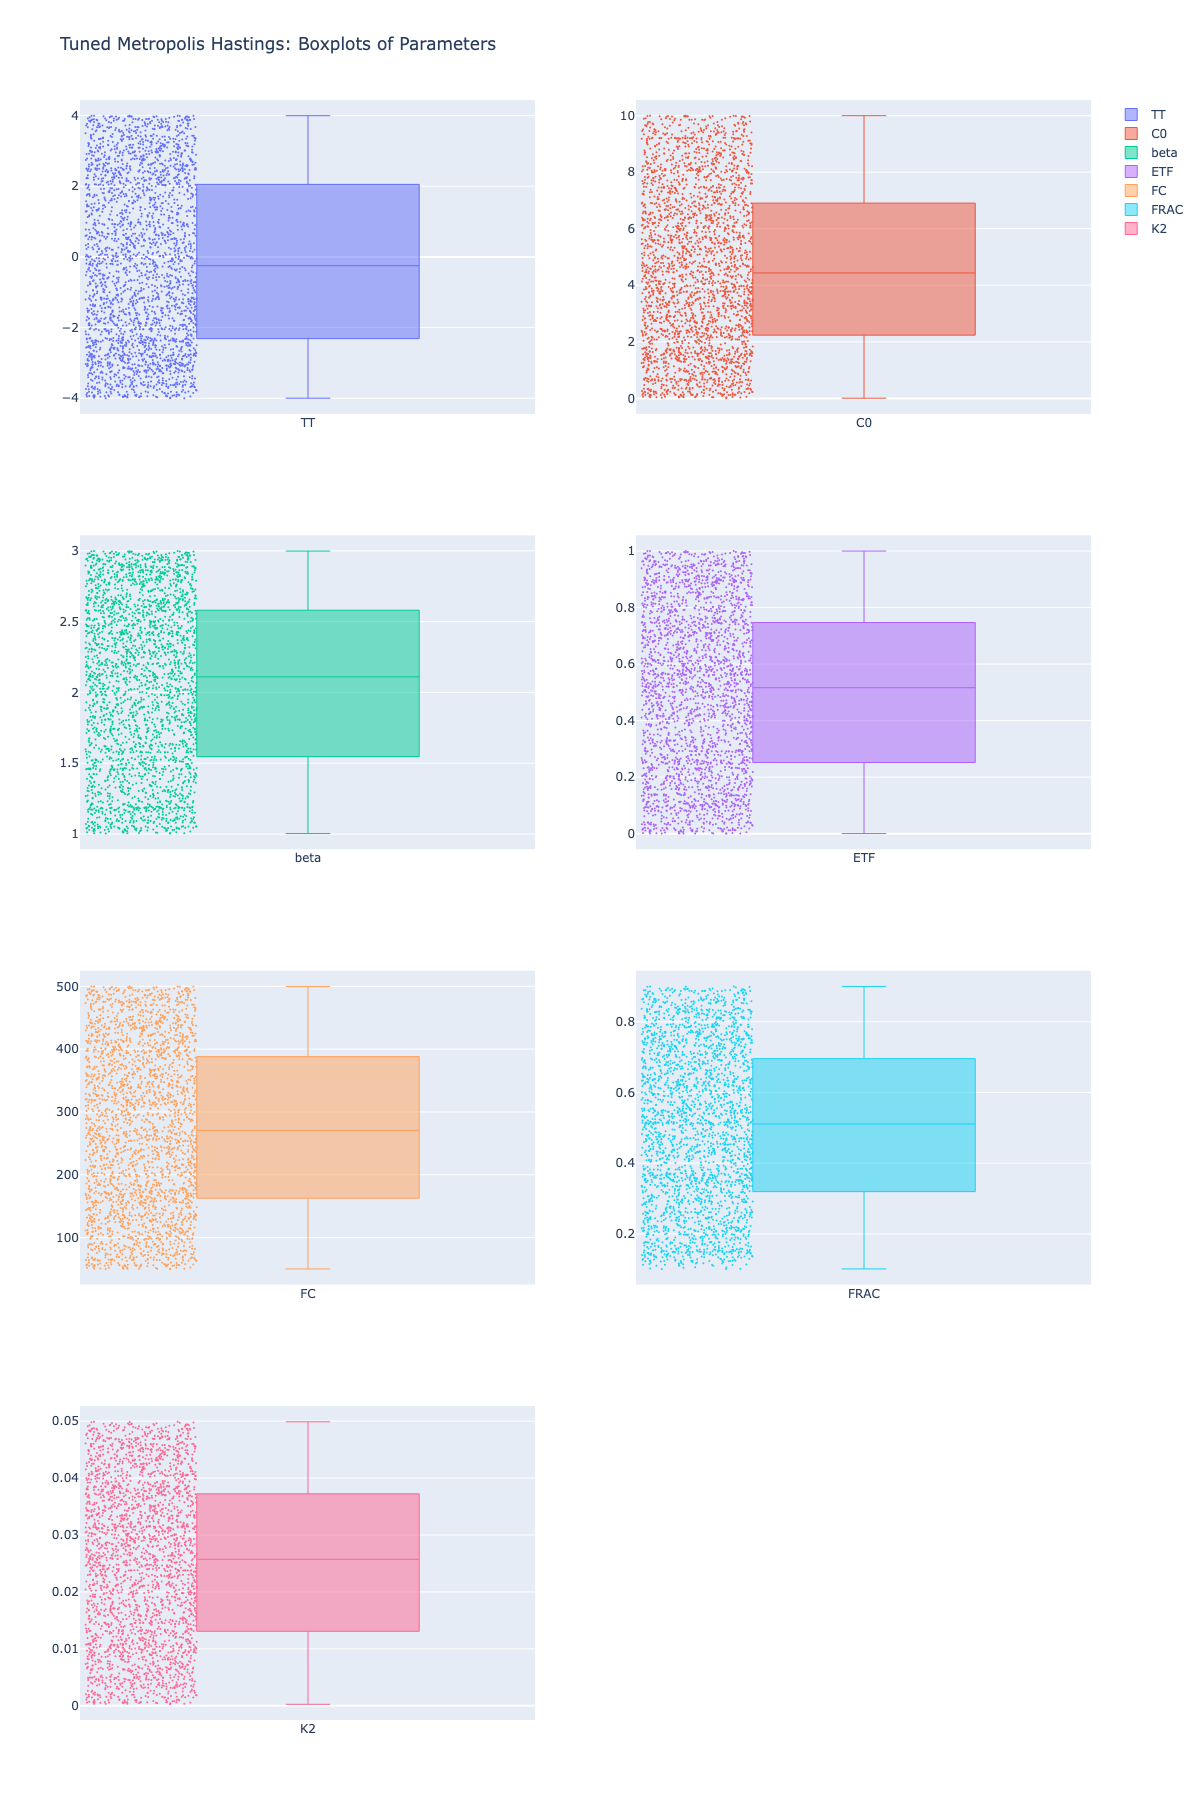
\includegraphics[width=1\textwidth]{figures/basic_mh/tuned_mh/tuned_mh_boxplot.png}
    \captionsetup{width=.8\textwidth}
    \caption{Boxplots of the generated posterior samples of each parameter calibrated by the Metropolis-Hastings algorithm with tuned input algorithm parameters}
    \label{fig:enter-label}
\end{figure}


From these generated samples, we retrieve the following result of the Bayesian inference problem shown in Figure 5.19.

\begin{figure}[H]
    \centering
    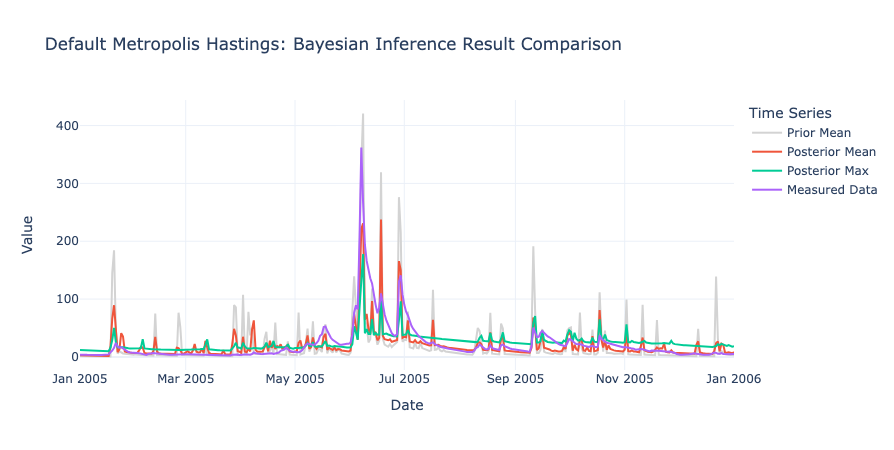
\includegraphics[width=0.8\textwidth] {figures/basic_mh/tuned_mh/tuned_mh_bayes.png}
    \captionsetup{width=.8\textwidth}
    \caption{Comparison of Bayesian inference results of the Metropolis-Hastings with tuned input algorithm parameters}
    \label{fig:enter-label}
\end{figure}

To evaluate the result, we keep using the metrics that were calculated before for the model using the knowledged-based set of input algorithm parameters, namely RMSE and MAE. The same calculations are executed on the mean and the maximum of the inferred time series. The RMSE of the posterior mean is 21.974609013782757 and the MAE of the posterior mean is 11.457657543376751, whereas the RMSE of the posterior max is 24.458078992931487 and the MAE of the posterior max is 14.532783129590447. The model using the tuned input algorithm parameters performs better than the model using the knowledge-based input algorithm parameters in some metrics, but not the others. Besides, there is randomness in the Monte Carlo algorithm~\cite{monte_carlo_randomness}, which contributes to slightly different values in every single execution.

Therefore, to generalize the accuracy of the result, we run both models 100 times and gather the mean of all the metrics of the results.

\begin{center}
\begin{tabular}{@{}lcc@{}}
\toprule
\textbf{Metric} & \textbf{Knowledge-Based Posterior Mean} & \textbf{Tuned Posterior Mean} \\ \midrule
RMSE            & 22.122504129857315               & 22.124942509212538                  \\
MAE             & 11.400067417022779               & 11.600318945622558              \\ \bottomrule
\end{tabular}
\end{center}




From this table, the knowledge-based input algorithm parameters achieve an all-around better performance, but not by much. While the RMSE does not differ from each other that much, the knowledge-based input algorithm parameters provide a slightly lower MAE. This might be the case that the inferred time series run by the model using the tuned input algorithm parameters performs slightly poorer in predicting extreme data points.

Therefore, we select the knowledge-based input algorithm parameters as the default input algorithm parameters for the Metropolis-Hastings algorithm for further usage in this paper.



